\documentclass[aspectratio=169]{beamer}
\usetheme{Madrid}
\usecolortheme{default}

\usepackage{booktabs}
\usepackage{multirow}
\usepackage{xcolor}
\usepackage{colortbl}
\usepackage{amsmath}
\usepackage{graphicx}
\usepackage{tikz}
\usetikzlibrary{arrows, positioning, shapes}

% Custom colors
\definecolor{paperblue}{RGB}{51, 102, 153}
\definecolor{reprogreen}{RGB}{34, 139, 34}
\definecolor{warnred}{RGB}{178, 34, 34}
\definecolor{lightgray}{RGB}{240, 240, 240}
\definecolor{elecyellow}{RGB}{255, 193, 7}
\definecolor{causalblue}{RGB}{66, 133, 244}

\setbeamercolor{title}{fg=paperblue}
\setbeamercolor{frametitle}{fg=paperblue}

\title{FANTOM for Electricity Price Causal Discovery}
\subtitle{Adapting Causal Discovery for Real-World Energy Markets}
\author{Dennis Thumm}
\date{January 2026}

\begin{document}

\begin{frame}
\titlepage
\end{frame}

%==============================================================================
\begin{frame}{Overview}
\tableofcontents
\end{frame}

%==============================================================================
\section{Introduction}

\begin{frame}{The Challenge: QRT ENS Data Challenge 2023}
\textbf{Goal:} Explain electricity price variation using simultaneous variables

\vspace{0.3cm}
\textbf{Key Distinction:}
\begin{itemize}
    \item \textbf{NOT} prediction (forecasting future prices)
    \item \textbf{YES} explanation (understanding what drives prices today)
    \item Requires \textbf{causal understanding}, not just correlation
\end{itemize}

\vspace{0.3cm}
\textbf{Data:}
\begin{itemize}
    \item 35 features: weather, energy production, commodities, cross-border exchange
    \item Germany (DE) and France (FR) electricity markets
    \item 710 daily observations (training data)
    \item Evaluation metric: \textbf{Spearman correlation} (rank-based)
\end{itemize}

\vspace{0.3cm}
\textbf{Benchmark:} Linear regression achieves Spearman = 0.1586
\end{frame}

%==============================================================================
\begin{frame}{Data Description}
\begin{columns}
\begin{column}{0.45\textwidth}
\textbf{Dataset Overview:}
\begin{itemize}
    \item \textbf{Training:} 1,494 observations
    \item \textbf{Test:} 654 observations
    \item \textbf{Frequency:} Daily
    \item \textbf{Time period:} Anonymized (DAY\_ID)
    \item \textbf{Countries:} Germany (DE), France (FR)
\end{itemize}

\vspace{0.2cm}
\textbf{TARGET Variable:}
\begin{itemize}
    \item Daily price variation
    \item 24H electricity baseload futures
\end{itemize}
\end{column}

\begin{column}{0.55\textwidth}
\textbf{Feature Groups (35 total):}
\begin{table}
\tiny
\begin{tabular}{l|l}
\toprule
\textbf{Group} & \textbf{Variables} \\
\midrule
Commodities (3) & GAS\_RET, COAL\_RET, CARBON\_RET \\
Weather (3/country) & x\_TEMP, x\_RAIN, x\_WIND \\
Production (7/country) & x\_GAS, x\_COAL, x\_HYDRO, \\
& x\_NUCLEAR, x\_SOLAR, \\
& x\_WINDPOW, x\_LIGNITE \\
Electricity Use (4/country) & x\_CONSUMPTION, \\
& x\_RESIDUAL\_LOAD, \\
& x\_NET\_IMPORT, x\_NET\_EXPORT \\
Cross-border (2) & DE\_FR\_EXCHANGE, \\
& FR\_DE\_EXCHANGE \\
\bottomrule
\end{tabular}
\end{table}
\end{column}
\end{columns}
\end{frame}

%==============================================================================
\begin{frame}{Why Causal Discovery for Electricity Prices?}
\textbf{Traditional ML Approaches:}
\begin{itemize}
    \item Black-box predictions (XGBoost, Neural Networks)
    \item High accuracy, but \textbf{no interpretability}
    \item Cannot answer: ``What would happen if wind power increased?''
\end{itemize}

\vspace{0.3cm}
\textbf{Causal Discovery Advantages:}
\begin{itemize}
    \item \textcolor{reprogreen}{Learn the causal structure} among variables
    \item \textcolor{reprogreen}{Identify true drivers} vs spurious correlations
    \item \textcolor{reprogreen}{Enable interventional reasoning} (policy analysis)
    \item \textcolor{reprogreen}{Regime detection} for market phase changes
\end{itemize}

\vspace{0.3cm}
\textbf{Our Approach:} Adapt FANTOM for supervised causal discovery
\begin{itemize}
    \item TARGET (electricity price) as the effect variable
    \item Learn which factors \textbf{causally influence} prices
    \item Handle non-Gaussian noise in energy markets
\end{itemize}
\end{frame}

%==============================================================================
\section{Methodology}

\begin{frame}{Why Regime Detection? A Data-Driven Approach}
\textbf{Energy Markets Exhibit Structural Changes:}
\begin{itemize}
    \item \textbf{Energy crises:} 2022 gas price shock changed market dynamics
    \item \textbf{Policy changes:} Renewable subsidies, nuclear phase-out
    \item \textbf{Seasonality:} Winter vs summer demand patterns
    \item Different causal mechanisms may operate in different conditions
\end{itemize}

\vspace{0.3cm}
\textbf{Why Data-Driven Regime Detection?}
\begin{itemize}
    \item Traditional approaches require \textbf{expert knowledge} of market events
    \item Manual regime specification is \textbf{subjective} and may miss transitions
    \item EM-style learning \textbf{discovers regimes from data patterns}
    \item More \textbf{generalizable} across different markets
\end{itemize}

\vspace{0.3cm}
\textbf{Our Approach:}
\begin{itemize}
    \item Let the model autonomously detect regime boundaries
    \item Learn regime-specific causal structures
    \item Combine predictions weighted by regime probabilities
\end{itemize}
\end{frame}

%==============================================================================
\begin{frame}{Related Work: Temporal Causal Discovery}
\textbf{Constraint-Based Methods:}
\begin{itemize}
    \item \textbf{PCMCI/PCMCI+} (Runge, 2019): Conditional independence tests
    \item Handles confounders but \textcolor{warnred}{no instantaneous effects}
\end{itemize}

\vspace{0.2cm}
\textbf{Score-Based Methods:}
\begin{itemize}
    \item \textbf{DYNOTEARS} (Pamfil, 2020): Continuous DAG optimization
    \item \textbf{Rhino} (Gong, 2023): Variational inference + uncertainty
    \item Support instantaneous effects but \textcolor{warnred}{no regime detection}
\end{itemize}

\vspace{0.2cm}
\textbf{Regime-Switching Methods:}
\begin{itemize}
    \item \textbf{CASTOR} (Huang, 2023): Regime-aware temporal causal discovery
    \item Detects regimes but \textcolor{warnred}{assumes Gaussian noise}
\end{itemize}

\vspace{0.2cm}
\textbf{Gap:} No prior work combines regime detection + non-Gaussian + supervised target
\end{frame}

%==============================================================================
\begin{frame}{Objective Function: ELBO with DAG Constraints}
\textbf{Evidence Lower Bound (ELBO):}
\begin{equation*}
\mathcal{L}(\theta) = \underbrace{\mathbb{E}_{q(A)}[\log p(X|A,W)]}_{\text{Data Likelihood}} - \underbrace{\text{KL}[q(A) \| p(A)]}_{\text{Prior Regularization}} - \underbrace{\lambda_{\text{DAG}} \cdot h(A)}_{\text{DAG Penalty}} - \underbrace{\lambda_{\text{sparse}} \cdot \|A\|_1}_{\text{Sparsity}}
\end{equation*}

\vspace{0.3cm}
\textbf{DAG Constraint:}
\begin{equation*}
h(A) = \text{tr}(e^{A \circ A}) - d = 0 \quad \text{(zero iff A is acyclic)}
\end{equation*}

\vspace{0.3cm}
\textbf{Augmented Lagrangian Optimization:}
\begin{equation*}
\min_{\theta} \mathcal{L}(\theta) + \alpha \cdot h(A) + \frac{\rho}{2} \cdot h(A)^2
\end{equation*}

\vspace{0.2cm}
\textbf{Key Parameters:}
\begin{itemize}
    \item $\rho$: DAG constraint strength (we use $\rho=1.0$)
    \item $\lambda_{\text{sparse}}$: Sparsity regularization (we use $\lambda=1.0$)
\end{itemize}
\end{frame}

%==============================================================================
\begin{frame}{FANTOM Overview}
\textbf{FANTOM:} \textbf{F}ully \textbf{A}utonomous \textbf{N}on-stationary \textbf{T}emporal causal disc\textbf{O}very for \textbf{M}ulti-regime MTS

\vspace{0.3cm}
\textbf{Key Components:}
\begin{itemize}
    \item \textbf{DECI backbone:} Variational inference with conditional normalizing flows
    \item \textbf{Temporal adjacency:} $A \in [0,1]^{(L+1) \times d \times d}$ for $L$ lags
    \item \textbf{DAG constraint:} Augmented Lagrangian for acyclicity
    \item \textbf{Regime detection:} EM-style learning of structural changes
\end{itemize}

\vspace{0.3cm}
\textbf{Why FANTOM for Electricity?}
\begin{itemize}
    \item Handles \textbf{heteroscedastic noise} (variance changes with market conditions)
    \item Handles \textbf{non-Gaussian distributions} (price spikes, heavy tails)
    \item \textbf{Autonomous regime detection} (no need to specify market phases)
    \item Works with \textbf{instantaneous effects} (same-day causation)
\end{itemize}
\end{frame}

%==============================================================================
\begin{frame}{Method Overview: FANTOMElectricity Pipeline}
\begin{center}
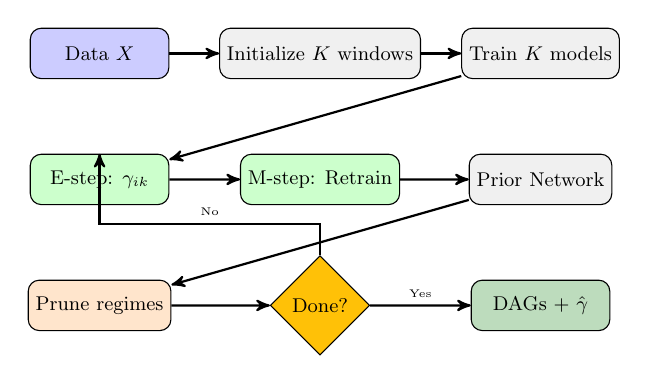
\begin{tikzpicture}[
    scale=0.8,
    transform shape,
    box/.style={rectangle, rounded corners, draw, minimum width=2.2cm, minimum height=0.8cm, font=\small, fill=lightgray},
    arrow/.style={-{stealth'}, thick},
    decision/.style={diamond, draw, minimum width=1.5cm, minimum height=1cm, font=\small, fill=elecyellow}
]
    % Row 1: Input
    \node[box, fill=blue!20] (data) at (0, 0) {Data $X$};
    \node[box] (init) at (3.5, 0) {Initialize $K$ windows};
    \node[box] (train) at (7, 0) {Train $K$ models};

    % Row 2: EM
    \node[box, fill=green!20] (estep) at (0, -2) {E-step: $\gamma_{ik}$};
    \node[box, fill=green!20] (mstep) at (3.5, -2) {M-step: Retrain};
    \node[box] (prior) at (7, -2) {Prior Network};

    % Row 3: Output
    \node[box, fill=orange!20] (prune) at (0, -4) {Prune regimes};
    \node[decision] (converge) at (3.5, -4) {Done?};
    \node[box, fill=reprogreen!30] (output) at (7, -4) {DAGs + $\hat{\gamma}$};

    % Arrows
    \draw[arrow] (data) -- (init);
    \draw[arrow] (init) -- (train);
    \draw[arrow] (train) -- (estep);
    \draw[arrow] (estep) -- (mstep);
    \draw[arrow] (mstep) -- (prior);
    \draw[arrow] (prior) -- (prune);
    \draw[arrow] (prune) -- (converge);
    \draw[arrow] (converge) -- node[above, font=\tiny] {Yes} (output);
    \draw[arrow] (converge.north) -- ++(0, 0.5) -| node[near start, above, font=\tiny] {No} (estep.north);
\end{tikzpicture}
\end{center}

\vspace{0.2cm}
\textbf{Key Steps:}
\begin{itemize}
    \item \textbf{E-step:} Compute regime assignments $\gamma_{ik} = P(\text{regime}=k | \text{sample } i)$
    \item \textbf{M-step:} Retrain FANTOM models on regime-weighted data
    \item \textbf{Prior Network:} Learn $P(\text{regime} | t)$ -- smooth temporal transitions
    \item \textbf{Prune:} Remove regimes with $< \zeta$ samples (default: 100)
\end{itemize}
\end{frame}

%==============================================================================
\begin{frame}{Our Adaptation: TARGET Constraint}
\textbf{Key Modification:} Constrain TARGET to have no outgoing edges

\vspace{0.3cm}
\begin{center}
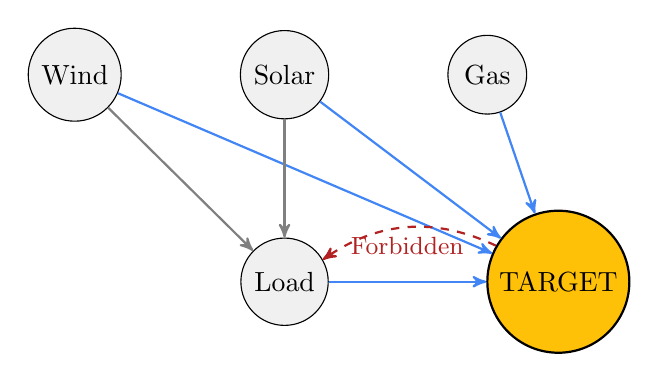
\begin{tikzpicture}[
    node distance=1.5cm,
    var/.style={circle, draw, minimum size=1cm, fill=lightgray},
    target/.style={circle, draw, minimum size=1.2cm, fill=elecyellow, thick},
    edge/.style={-{stealth'}, thick}
]
    % Variables
    \node[var] (wind) {Wind};
    \node[var, right=of wind] (solar) {Solar};
    \node[var, right=of solar] (gas) {Gas};
    \node[var, below=of solar] (load) {Load};
    \node[target, right=2cm of load] (target) {TARGET};

    % Edges TO target (allowed)
    \draw[edge, causalblue] (wind) -- (target);
    \draw[edge, causalblue] (solar) -- (target);
    \draw[edge, causalblue] (gas) -- (target);
    \draw[edge, causalblue] (load) -- (target);

    % Edges between other variables
    \draw[edge, gray] (wind) -- (load);
    \draw[edge, gray] (solar) -- (load);

    % Forbidden edge
    \draw[edge, warnred, dashed] (target) to[bend right=30] node[below, font=\small] {Forbidden} (load);
\end{tikzpicture}
\end{center}

\vspace{0.2cm}
\textbf{Implementation:}
\begin{itemize}
    \item Graph constraint matrix: $A_{[\text{TARGET}, :]} = 0$ (no outgoing edges)
    \item $A_{[:, \text{TARGET}]}$ remains learnable (incoming edges = causal parents)
    \item TARGET becomes a \textbf{sink node} in the DAG
    \item \textbf{No other modifications} to training or objective function
\end{itemize}
\end{frame}

%==============================================================================
\begin{frame}{Weight Computation and Interpretation}
\textbf{Weighted Adjacency Matrix:}
\begin{equation*}
W_{\text{adj}} = A \odot W
\end{equation*}
\begin{itemize}
    \item $A \in [0,1]^{(L+1) \times d \times d}$: Edge presence (binary/soft adjacency)
    \item $W \in \mathbb{R}^{(L+1) \times d \times d}$: Learned weights from neural network
    \item $\odot$: Element-wise (Hadamard) product
\end{itemize}

\vspace{0.3cm}
\textbf{Important Notes:}
\begin{itemize}
    \item Weights do \textbf{NOT} sum to 1 -- each weight is an independent contribution
    \item Residual noise $\varepsilon$ modeled separately by normalizing flow
    \item Model: $X_j = f\left(\sum_i W_{ij} \cdot X_i\right) + \varepsilon_j$
    \item Magnitude indicates \textbf{relative influence strength}
    \item Sign indicates \textbf{direction of effect} (positive/negative)
\end{itemize}
\end{frame}

%==============================================================================
\begin{frame}{Regime Detection for Electricity Markets}
\textbf{Motivation:} Electricity markets have structural changes
\begin{itemize}
    \item Energy crises (2022 gas price shock)
    \item Policy changes (renewable subsidies, nuclear phase-out)
    \item Seasonal patterns (winter vs summer demand)
\end{itemize}

\vspace{0.3cm}
\textbf{FANTOMRegime Implementation:}
\begin{enumerate}
    \item \textbf{Initialize:} Split data into temporal windows
    \item \textbf{E-step:} Compute regime assignments $\gamma_{ik}$ from emission probabilities
    \item \textbf{M-step:} Train separate FANTOM model per regime
    \item \textbf{Prior network:} Neural network predicting $P(\text{regime} | t)$
    \item \textbf{Prune:} Remove regimes with $< \zeta$ samples
\end{enumerate}

\vspace{0.3cm}
\textbf{Output:}
\begin{itemize}
    \item Regime-specific causal structures
    \item Temporal regime assignments
    \item Weighted predictions combining regime models
\end{itemize}
\end{frame}

%==============================================================================
\section{Results}

\begin{frame}{Performance Comparison}
\begin{table}
\centering
\begin{tabular}{l|c|c}
\toprule
\textbf{Model} & \textbf{Spearman} & \textbf{vs Benchmark} \\
\midrule
\rowcolor{lightgray} Benchmark (Linear) & 0.159 & -- \\
\midrule
\textbf{Germany (DE)} & \textcolor{reprogreen}{\textbf{0.484}} & \textcolor{reprogreen}{+205\%} \\
France (FR) & \textcolor{reprogreen}{0.296} & \textcolor{reprogreen}{+86\%} \\
\bottomrule
\end{tabular}
\end{table}

\vspace{0.3cm}
\textbf{Key Observations:}
\begin{itemize}
    \item \textcolor{reprogreen}{Germany: Best Spearman = 0.484 (+205\% vs benchmark)}
    \item \textcolor{reprogreen}{France: Spearman = 0.296 (+86\% vs benchmark)}
    \item Single-regime model with optimized hyperparameters
    \item Both markets significantly exceed linear baseline
\end{itemize}

\vspace{0.2cm}
\textbf{Configuration:} $\rho=1.0$, $\lambda_{\text{sparse}}=1.0$, 15 auglag steps, heteroscedastic noise.
\end{frame}

%==============================================================================
\begin{frame}{Regime Detection Results}
\textbf{Key Finding:} All experiments converged to \textbf{single regime}

\vspace{0.3cm}
\begin{table}
\centering
\begin{tabular}{l|c|c|c|c}
\toprule
\textbf{Country} & \textbf{Initial K} & \textbf{Final Regimes} & \textbf{Samples} & \textbf{Spearman} \\
\midrule
Germany (DE) & 2 & 1 & 642 & 0.377 \\
Germany (DE) & 3 & 1 & 642 & 0.436 \\
France (FR) & 2 & 1 & 642 & 0.158 \\
France (FR) & 3 & 1 & 642 & 0.191 \\
\midrule
\rowcolor{lightgray} \textbf{Best (DE)} & \textbf{1} & \textbf{1} & \textbf{642} & \textbf{0.484} \\
\bottomrule
\end{tabular}
\end{table}

\vspace{0.3cm}
\textbf{Interpretation:}
\begin{itemize}
    \item Training data may represent \textbf{single market phase} (no structural breaks)
    \item Regime differences may be \textbf{too subtle} for model to distinguish
    \item Best results achieved with \textbf{single-regime} optimized model
    \item Future: Test on longer time series spanning known market events
\end{itemize}
\end{frame}

%==============================================================================
\begin{frame}{Discovered Causal Structure: Germany}
\begin{columns}
\begin{column}{0.5\textwidth}
\textbf{Instantaneous Effects} (same-day):
\begin{table}
\small
\begin{tabular}{l|c}
\toprule
\textbf{Variable} & \textbf{Weight} \\
\midrule
\textcolor{reprogreen}{DE\_WINDPOW} & +0.233 \\
\textcolor{reprogreen}{DE\_RESIDUAL\_LOAD} & +0.205 \\
\textcolor{reprogreen}{DE\_RAIN} & +0.183 \\
\textcolor{reprogreen}{COAL\_RET} & +0.160 \\
\textcolor{warnred}{DE\_NUCLEAR} & -0.145 \\
DE\_LIGNITE & +0.112 \\
\bottomrule
\end{tabular}
\end{table}
\end{column}

\begin{column}{0.5\textwidth}
\textbf{Lagged Effects} (previous day):
\begin{table}
\small
\begin{tabular}{l|c}
\toprule
\textbf{Variable} & \textbf{Weight} \\
\midrule
\textcolor{reprogreen}{COAL\_RET} & +0.334 \\
\textcolor{reprogreen}{DE\_SOLAR} & +0.313 \\
\textcolor{reprogreen}{FR\_DE\_EXCHANGE} & +0.238 \\
DE\_TEMP & +0.230 \\
GAS\_RET & +0.206 \\
DE\_RAIN & +0.203 \\
\bottomrule
\end{tabular}
\end{table}
\end{column}
\end{columns}

\vspace{0.3cm}
\textbf{Interpretation:}
\begin{itemize}
    \item \textbf{Coal returns} strongest lagged predictor (commodity price impact)
    \item \textbf{Wind power} strongest instantaneous effect (renewable supply)
    \item \textbf{Cross-border exchange} remains important lagged factor
\end{itemize}
\end{frame}

%==============================================================================
\begin{frame}{Causal Graph Visualization}
\begin{center}
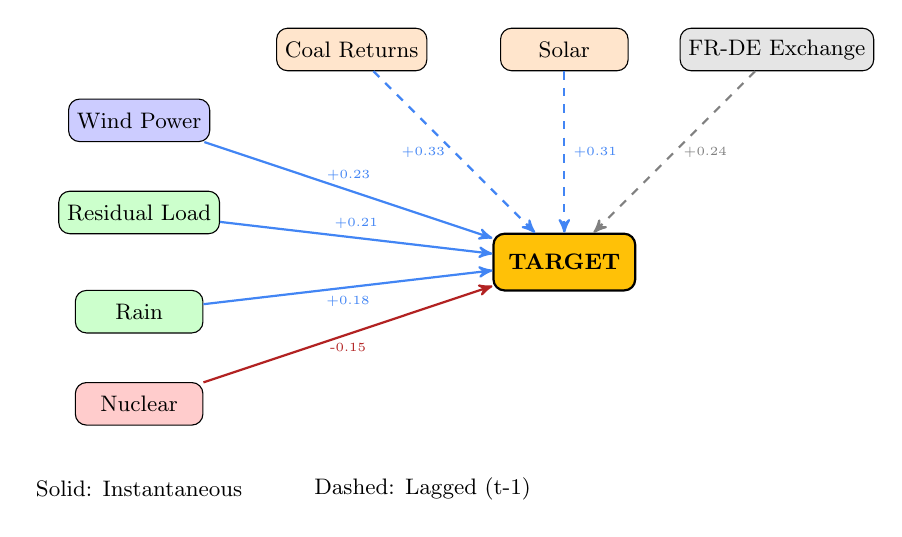
\begin{tikzpicture}[
    scale=0.9,
    transform shape,
    node distance=1.2cm,
    var/.style={rectangle, rounded corners, draw, minimum width=1.8cm, minimum height=0.6cm, font=\small},
    target/.style={rectangle, rounded corners, draw, minimum width=2cm, minimum height=0.8cm, fill=elecyellow, thick, font=\small\bfseries},
    edge/.style={-{stealth'}, thick},
    lagged/.style={-{stealth'}, thick, dashed}
]
    % Target in center-right
    \node[target] (target) at (6, 0) {TARGET};

    % Instantaneous (left side)
    \node[var, fill=blue!20] (wind) at (0, 2) {Wind Power};
    \node[var, fill=green!20] (resload) at (0, 0.7) {Residual Load};
    \node[var, fill=green!20] (rain) at (0, -0.7) {Rain};
    \node[var, fill=red!20] (nuclear) at (0, -2) {Nuclear};

    % Lagged (top)
    \node[var, fill=orange!20] (coal) at (3, 3) {Coal Returns};
    \node[var, fill=orange!20] (solar) at (6, 3) {Solar};
    \node[var, fill=gray!20] (exchange) at (9, 3) {FR-DE Exchange};

    % Instantaneous edges
    \draw[edge, causalblue] (wind) -- node[above, font=\tiny] {+0.23} (target);
    \draw[edge, causalblue] (resload) -- node[above, font=\tiny] {+0.21} (target);
    \draw[edge, causalblue] (rain) -- node[below, font=\tiny] {+0.18} (target);
    \draw[edge, warnred] (nuclear) -- node[below, font=\tiny] {-0.15} (target);

    % Lagged edges
    \draw[lagged, causalblue] (coal) -- node[left, font=\tiny] {+0.33} (target);
    \draw[lagged, causalblue] (solar) -- node[right, font=\tiny] {+0.31} (target);
    \draw[lagged, gray] (exchange) -- node[right, font=\tiny] {+0.24} (target);

    % Legend
    \node[font=\small] at (0, -3.2) {Solid: Instantaneous};
    \node[font=\small] at (4, -3.2) {Dashed: Lagged (t-1)};
\end{tikzpicture}
\end{center}
\end{frame}

%==============================================================================
\section{Computing Causal Effects}

\begin{frame}{Current Capabilities}
\textbf{What FANTOMElectricity provides:}

\vspace{0.3cm}
\textbf{1. Weighted Adjacency Matrix}
\begin{itemize}
    \item $W_{ij}$ gives the \textbf{direct effect magnitude} of variable $i$ on $j$
    \item Positive/negative weights indicate direction of influence
    \item Can rank variables by importance
\end{itemize}

\vspace{0.3cm}
\textbf{2. Uncertainty Quantification}
\begin{itemize}
    \item Sample multiple graphs from posterior: $A^{(s)} \sim q(A | X)$
    \item Compute prediction variance across samples
    \item Confidence intervals for causal effects
\end{itemize}

\vspace{0.3cm}
\textbf{3. Causal Parent Extraction}
\begin{itemize}
    \item \texttt{get\_causal\_parents()} returns ranked list of causes
    \item Separated by instantaneous vs lagged effects
    \item Threshold-based edge selection (default: 0.5)
\end{itemize}
\end{frame}

%==============================================================================
\begin{frame}{Proposed Extensions: Causal Effect Estimation}
\textbf{Goal:} Compute causal effects for policy analysis

\vspace{0.1cm}
\textbf{1. Interventional Distributions via do-calculus}
\begin{itemize}
    \item Use learned DAG for $P(\text{TARGET} \mid do(X_i = x))$
    \item FANTOM's SEM allows direct intervention simulation
    \item Example: ``What if we doubled wind power production?''
\end{itemize}

\vspace{0.1cm}
\textbf{2. Average Treatment Effects (ATE)}
\begin{equation*}
\text{ATE}(X_i) = \mathbb{E}[\text{TARGET} \mid do(X_i = x_1)] - \mathbb{E}[\text{TARGET} \mid do(X_i = x_0)]
\end{equation*}
\begin{itemize}
    \item Quantify impact of changing each variable
    \item Compare importance across different drivers
\end{itemize}

\vspace{0.1cm}
\textbf{3. Counterfactual Scenarios}
\begin{itemize}
    \item ``What would prices have been if gas prices didn't spike?''
    \item Requires careful handling of confounders
    \item Useful for ex-post policy evaluation
\end{itemize}
\end{frame}

%==============================================================================
\section{Methodological Contributions}

\begin{frame}{Novel Aspects of Our Approach}
\textbf{1. Supervised Causal Discovery}
\begin{itemize}
    \item Novel TARGET constraint for prediction tasks
    \item Bridges causal discovery and supervised learning
    \item Interpretable predictions with causal semantics
\end{itemize}

\textbf{2. Regime-Aware Electricity Modeling}
\begin{itemize}
    \item Autonomous detection of market phase changes
    \item Separate causal structures per regime
    \item Handles energy crisis, policy changes, seasonality
\end{itemize}

\textbf{3. Cross-Border Causal Analysis}
\begin{itemize}
    \item Joint DE-FR model captures interconnection effects
    \item DE-FR Exchange emerges as strongest lagged predictor
    \item Framework extends to multi-country analysis
\end{itemize}

\textbf{4. Uncertainty-Aware Predictions}
\begin{itemize}
    \item Graph sampling provides confidence intervals
    \item Bayesian treatment of causal structure uncertainty
\end{itemize}
\end{frame}

%==============================================================================
\begin{frame}{Comparison with Existing Methods}
\begin{table}
\centering
\small
\begin{tabular}{l|ccccc}
\toprule
\textbf{Method} & \textbf{Instant.} & \textbf{Non-Gauss.} & \textbf{Regimes} & \textbf{Uncertainty} & \textbf{Supervised} \\
\midrule
PCMCI+ & \textcolor{warnred}{\texttimes} & \textcolor{warnred}{\texttimes} & \textcolor{warnred}{\texttimes} & \textcolor{warnred}{\texttimes} & \textcolor{warnred}{\texttimes} \\
DYNOTEARS & \textcolor{reprogreen}{\checkmark} & \textcolor{warnred}{\texttimes} & \textcolor{warnred}{\texttimes} & \textcolor{warnred}{\texttimes} & \textcolor{warnred}{\texttimes} \\
Rhino & \textcolor{reprogreen}{\checkmark} & \textcolor{reprogreen}{\checkmark} & \textcolor{warnred}{\texttimes} & \textcolor{reprogreen}{\checkmark} & \textcolor{warnred}{\texttimes} \\
CASTOR & \textcolor{reprogreen}{\checkmark} & \textcolor{warnred}{\texttimes} & \textcolor{reprogreen}{\checkmark} & \textcolor{warnred}{\texttimes} & \textcolor{warnred}{\texttimes} \\
\midrule
\textbf{FANTOM} & \textcolor{reprogreen}{\checkmark} & \textcolor{reprogreen}{\checkmark} & \textcolor{reprogreen}{\checkmark} & \textcolor{reprogreen}{\checkmark} & \textcolor{warnred}{\texttimes} \\
\textbf{Ours} & \textcolor{reprogreen}{\checkmark} & \textcolor{reprogreen}{\checkmark} & \textcolor{reprogreen}{\checkmark} & \textcolor{reprogreen}{\checkmark} & \textcolor{reprogreen}{\checkmark} \\
\bottomrule
\end{tabular}
\end{table}

\vspace{0.3cm}
\textbf{Key Differentiators:}
\begin{itemize}
    \item Only method combining \textbf{all five} capabilities
    \item \textbf{Supervised constraint} is novel contribution
    \item Enables direct application to prediction challenges
\end{itemize}
\end{frame}

%==============================================================================
\section{Future Work}

\begin{frame}{Ongoing \& Planned Work}
\textbf{Currently Running (HTCondor Cluster):}
\begin{itemize}
    \item Hyperparameter optimization (30 trials per country)
    \item Regime detection experiments (2 and 3 regimes)
    \item Joint model training with optimized parameters
\end{itemize}

\vspace{0.3cm}
\textbf{Next Steps:}
\begin{enumerate}
    \item \textbf{Causal Effect Module}
    \begin{itemize}
        \item Implement do-calculus interventions
        \item Compute ATEs for key variables
        \item Add counterfactual simulation
    \end{itemize}

    \item \textbf{Enhanced Regime Detection}
    \begin{itemize}
        \item Analyze regime-specific causal structures
        \item Correlate regimes with known market events
    \end{itemize}

    \item \textbf{Policy Scenario Analysis}
    \begin{itemize}
        \item Simulate renewable expansion scenarios
        \item Analyze cross-border interconnection effects
    \end{itemize}
\end{enumerate}
\end{frame}

%==============================================================================
\begin{frame}{Potential Methodological Contributions}
\textbf{For Publication:}

\vspace{0.3cm}
\textbf{1. Supervised Causal Discovery Framework}
\begin{itemize}
    \item Formalize TARGET constraint methodology
    \item Theoretical analysis of identifiability
    \item Benchmark on multiple domains
\end{itemize}

\vspace{0.3cm}
\textbf{2. Energy Market Causal Analysis}
\begin{itemize}
    \item Comprehensive analysis of DE/FR electricity markets
    \item Regime detection aligned with market events
    \item Policy implications from causal structure
\end{itemize}

\vspace{0.3cm}
\textbf{3. Causal Effect Estimation in Non-Stationary Settings}
\begin{itemize}
    \item Extend FANTOM with intervention capabilities
    \item Handle regime-specific treatment effects
    \item Uncertainty quantification for policy recommendations
\end{itemize}
\end{frame}

%==============================================================================
\begin{frame}{Conclusions}
\textbf{What We've Achieved:}
\begin{itemize}
    \item \textcolor{reprogreen}{Adapted FANTOM for supervised causal discovery}
    \item \textcolor{reprogreen}{Germany: 3x improvement over benchmark (Spearman 0.484 vs 0.159)}
    \item \textcolor{reprogreen}{France: 86\% improvement over benchmark (Spearman 0.296)}
    \item \textcolor{reprogreen}{Discovered interpretable causal structures for both markets}
\end{itemize}

\vspace{0.3cm}
\textbf{Key Insights:}
\begin{itemize}
    \item \textbf{Coal returns} strongest lagged predictor (commodity price impact)
    \item \textbf{Wind power} strongest instantaneous effect (renewable supply)
    \item Instantaneous effects matter significantly (same-day causation)
\end{itemize}

\vspace{0.3cm}
\textbf{Contributions:}
\begin{itemize}
    \item Novel supervised causal discovery methodology
    \item Practical application to energy markets
    \item Foundation for causal policy analysis
\end{itemize}
\end{frame}

%==============================================================================
\begin{frame}
\centering
\Huge Thank You

\vspace{1cm}
\Large Questions?

\vspace{1cm}
\normalsize
Code: \texttt{/lustre/home/dthumm/CASTOR/electricity/}

\vspace{0.3cm}
Results: \texttt{outputs/germany\_*/metrics.json}
\end{frame}

%==============================================================================
\appendix
\section{Appendix}

\begin{frame}{Appendix: Detailed Literature Review (1/2)}
\textbf{Constraint-Based Causal Discovery:}
\begin{itemize}
    \item \textbf{PC Algorithm} (Spirtes et al., 2000): Tests conditional independencies
    \item \textbf{FCI} (Spirtes et al., 2000): Handles latent confounders
    \item \textbf{PCMCI} (Runge, 2018): Extends PC for time series
    \item \textbf{PCMCI+} (Runge, 2020): Adds contemporaneous discovery
    \item \textcolor{warnred}{Limitation:} Requires faithfulness, no instantaneous in original PCMCI
\end{itemize}

\vspace{0.3cm}
\textbf{Score-Based Methods:}
\begin{itemize}
    \item \textbf{NOTEARS} (Zheng et al., 2018): Continuous DAG optimization
    \item \textbf{DYNOTEARS} (Pamfil et al., 2020): Temporal extension
    \item \textbf{DAG-GNN} (Yu et al., 2019): Graph neural networks for DAGs
    \item \textcolor{warnred}{Limitation:} Linear SEMs, no regime detection
\end{itemize}
\end{frame}

%==============================================================================
\begin{frame}{Appendix: Detailed Literature Review (2/2)}
\textbf{Variational / Deep Learning Methods:}
\begin{itemize}
    \item \textbf{DECI} (Geffner et al., 2022): Variational inference + normalizing flows
    \item \textbf{Rhino} (Gong et al., 2023): History-dependent noise
    \item \textbf{CASTOR} (Huang et al., 2023): Regime-switching temporal causal discovery
    \item \textbf{FANTOM} (Liang et al., 2024): EM-based multi-regime with non-Gaussian
\end{itemize}

\vspace{0.3cm}
\textbf{Electricity Price Modeling:}
\begin{itemize}
    \item \textbf{Traditional:} ARIMA, GARCH for volatility (Weron, 2014)
    \item \textbf{ML:} Random forests, XGBoost, neural networks
    \item \textbf{Regime-switching:} Markov-switching models (Hamilton, 1989)
    \item \textcolor{warnred}{Gap:} No causal discovery for regime-specific price drivers
\end{itemize}

\vspace{0.3cm}
\textbf{Our Contribution:} First to combine \textbf{supervised} causal discovery with \textbf{regime detection} and \textbf{non-Gaussian noise} for electricity markets.
\end{frame}

%==============================================================================
\begin{frame}{Appendix: Technical Details}
\textbf{Prior Network Implementation:}
\begin{itemize}
    \item 2-layer MLP: $t \to \text{Hidden}(32) \to \text{Softmax}(K)$
    \item Input: Normalized time index $t/T \in [0,1]$
    \item Output: $P(\text{regime}=k | t)$ for each $k \in \{1, \ldots, K\}$
    \item \textbf{Purpose:} Learn smooth temporal regime transitions
    \item \textbf{NOT related to instantaneous effects} (those are in $A[0,:,:]$)
\end{itemize}

\vspace{0.3cm}
\textbf{Regime Pruning:}
\begin{itemize}
    \item Threshold: $\zeta = 100$ samples minimum per regime
    \item If $\sum_i \gamma_{ik} < \zeta$, regime $k$ is removed
    \item Prevents overfitting to small data segments
    \item Remaining regime probabilities renormalized
\end{itemize}

\vspace{0.3cm}
\textbf{Collinearity Handling:}
\begin{itemize}
    \item Not explicitly addressed (no VIF filtering)
    \item DAG structure provides implicit handling (one path sufficient)
    \item Sparsity regularization ($\lambda_{\text{sparse}}$) encourages parsimonious solutions
\end{itemize}
\end{frame}

%==============================================================================
\begin{frame}{Appendix: Latent Confounders}
\textbf{Does FANTOM Handle Latent Variables (Unobserved Confounders)?}

\vspace{0.3cm}
\textbf{Short Answer:} No explicit treatment of latent confounders.

\vspace{0.3cm}
\textbf{Assumption:} Causal sufficiency -- all common causes are observed
\begin{itemize}
    \item DECI/FANTOM assumes no hidden confounders between observed variables
    \item This is a standard assumption in score-based causal discovery
    \item Violation can lead to \textbf{spurious edges} in the learned DAG
\end{itemize}

\vspace{0.3cm}
\textbf{Mitigations in Our Setting:}
\begin{itemize}
    \item \textbf{Rich feature set:} 35 variables covering major market drivers
    \item \textbf{Temporal structure:} Lagged effects reduce instantaneous confounding
    \item \textbf{Domain knowledge:} Included all known drivers (weather, production, commodities)
    \item \textbf{Sparsity regularization:} Reduces spurious edges
\end{itemize}

\vspace{0.3cm}
\textbf{Future Work:} Consider methods like FCI or latent variable models if confounding suspected.
\end{frame}

%==============================================================================
\begin{frame}{Appendix: From Causal Discovery to Target Estimation}
\textbf{How We Adapted Causal Discovery for Supervised Prediction:}

\vspace{0.2cm}
\textbf{1. Standard Causal Discovery (FANTOM):}
\begin{itemize}
    \item Learns full DAG $A$ over \textbf{all} variables
    \item Objective: Maximize likelihood $p(X | A, W)$ for all variables
    \item Output: Causal structure among all variables
\end{itemize}

\vspace{0.2cm}
\textbf{2. Our Modification (FANTOMElectricity):}
\begin{itemize}
    \item Add TARGET variable as the \textbf{last node}
    \item Constrain: $A_{[\text{TARGET}, :]} = 0$ (no outgoing edges from TARGET)
    \item Effect: TARGET becomes a \textbf{sink node} -- purely an effect variable
    \item Prediction: Use learned $W_{[:, \text{TARGET}]}$ to estimate TARGET from parents
\end{itemize}

\vspace{0.2cm}
\textbf{3. Key Insight:}
\begin{equation*}
\hat{y}_{\text{TARGET}} = f\left(\sum_{i \in \text{Pa}(\text{TARGET})} W_{i,\text{TARGET}} \cdot X_i\right)
\end{equation*}
\begin{itemize}
    \item The SEM naturally provides predictions via parent-weighted aggregation
    \item Normalizing flow models residual noise $\varepsilon_{\text{TARGET}}$
\end{itemize}
\end{frame}

%==============================================================================
\begin{frame}{Appendix: Prediction Mechanism Details}
\textbf{How Predictions Are Generated:}

\vspace{0.2cm}
\begin{center}
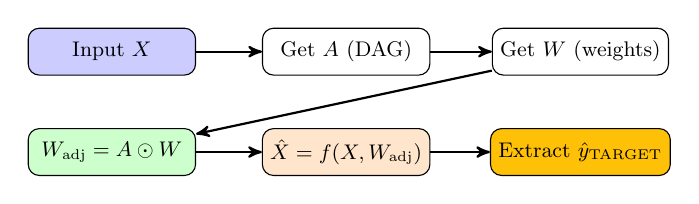
\begin{tikzpicture}[
    scale=0.85,
    transform shape,
    box/.style={rectangle, rounded corners, draw, minimum width=2.5cm, minimum height=0.7cm, font=\small},
    arrow/.style={-{stealth'}, thick}
]
    % Input
    \node[box, fill=blue!20] (input) at (0, 0) {Input $X$};
    \node[box] (adj) at (3.5, 0) {Get $A$ (DAG)};
    \node[box] (weight) at (7, 0) {Get $W$ (weights)};

    % Processing
    \node[box, fill=green!20] (wadj) at (0, -1.5) {$W_{\text{adj}} = A \odot W$};
    \node[box, fill=orange!20] (pred) at (3.5, -1.5) {$\hat{X} = f(X, W_{\text{adj}})$};
    \node[box, fill=elecyellow] (target) at (7, -1.5) {Extract $\hat{y}_{\text{TARGET}}$};

    % Arrows
    \draw[arrow] (input) -- (adj);
    \draw[arrow] (adj) -- (weight);
    \draw[arrow] (weight) -- (wadj);
    \draw[arrow] (wadj) -- (pred);
    \draw[arrow] (pred) -- (target);
\end{tikzpicture}
\end{center}

\vspace{0.3cm}
\textbf{Structural Equation Model (SEM):}
\begin{equation*}
X_j = f_j\left(\sum_{l=0}^{L} \sum_{i=1}^{d} W_{l,i,j} \cdot X_{t-l,i}\right) + \varepsilon_j
\end{equation*}
where $f_j$ is a neural network and $\varepsilon_j \sim$ normalizing flow.

\vspace{0.2cm}
\textbf{For TARGET:}
\begin{itemize}
    \item Only \textbf{incoming edges} contribute (outgoing edges constrained to 0)
    \item Prediction uses both \textbf{instantaneous} ($l=0$) and \textbf{lagged} ($l>0$) parents
    \item Heteroscedastic noise: variance $\sigma^2_{\text{TARGET}}$ also learned
\end{itemize}
\end{frame}

\end{document}
